\section{Risultati Sperimentali}
Verranno elencati in questa sezione i risultati sperimentali, essi
sono estremamente dipendenti da un numero enorme di fattori di configurazione
e utilizzo, prima fra tutti la scelta del metodo di improvvisazione da parte
del musicista.

\subsection{Algoritmo a scelta casuale}
L'algoritmo a scelta casuale, come indicato nella sezione \ref{sec:musician_think},
soffre estremamente la mancanza di un database di pattern ben costruito
\footnote{purtroppo sia per mancanza di conoscenza strumentale
(per esempio riguardo all'organo), sia per mancanza temporale,
il database è decisamente scarno per utilizzi più avanzati di un semplice
\textbf{proof of concepts}};
\\
\begin{figure}[H]
\centering
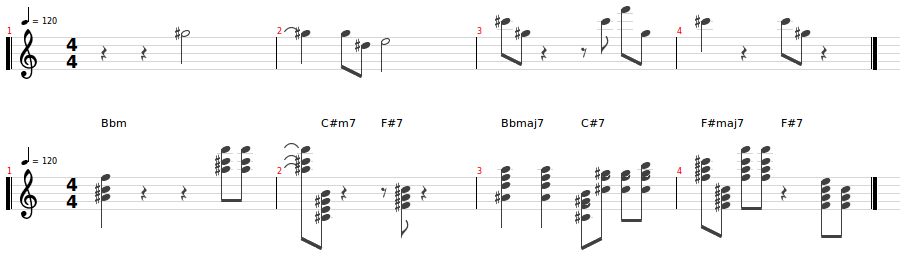
\includegraphics[width=\textwidth]{img/organmatch.png}
\caption{Improvvisazione con organo solista e pianoforte ad accordi.}
\end{figure}
questo si può notare immediatamente con un riscontro uditivo,
gli strumenti che possiedono un database di pattern ristretto tenderanno
a fare scelte sempre più casuali, dettate dalla granularità delle informazioni
presenti nel database, questa granularità è dettata tramite i \textbf{priorargs}
dal musicista in fase di computazione dell'improvvisazione.\\
Come possiamo notare dalla figura sovrastante, lo strumento con un numero ristretto
di pattern tenderà a suonare "peggio"\footnote{Associabile alla scarsa esperienza del musicista.}.
\\
\begin{figure}[H]
\centering
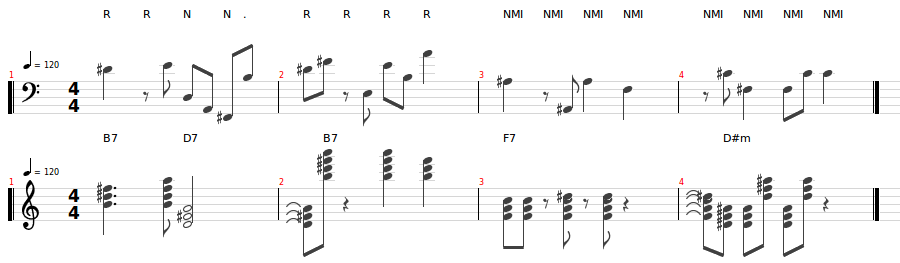
\includegraphics[width=\textwidth]{img/bassmatch.png}
\caption{Improvvisazione con linea di basso e pianoforte ad accordi.}
\end{figure}
In questa figura possiamo notare come strumenti con un numero maggiore di pattern siano
più "musicali" e meno "casuali" all'orecchio di un ascoltatore.\\
Inoltre possiamo notare come le basi teoriche musicali
di coesione tra i vari musicisti siano state ben implementate.

\subsection{Algoritmo a selezione naturale (genetico / evoluzionistico)}

L'algoritmo evoluzionistico segue invece scelte legate all'esperienza,
facendo apprendere al programma
\footnote{Uno dei possibili sviluppi futuri, se non il più stimolante da un
punto di vista informatico/tecnico è la possibilità di salvare l'apprendimento
di un singolo musicista nel database, in modo da creare apprendimenti misti,
o un apprendimento decisamente più profondo di un determinato genere.}
un determinato brano. \footnote{come indicato nella sezione \ref{sec:evol_alg}}
\\
Il problema della valutazione del singolo individuo (o run) è risultato, da un
punto di vista teorico, decisamente complesso.
Da un osservazione pratica/sperimentale,
questa tesi è stata confermata, i parametri di controllo della mutazione e
i parametri di valutazione dell'algoritmo genetico
\footnote{La funzione di valutazione,
senza avere input umani a runtime, usa meccanismi basati sulla norma 2
o distanza euclidea.}
sono risultati decisamente delicati, producendo risultati diversi ad una minima
variazione "dell'ago della bilancia".

\begin{figure}[H]
\centering
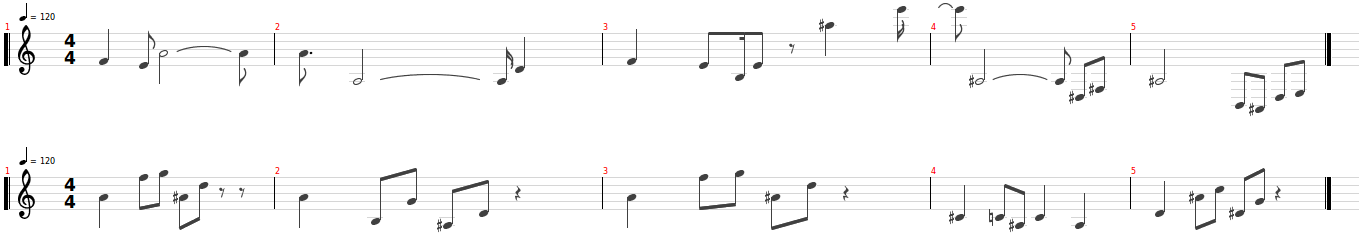
\includegraphics[width=\textwidth]{img/genmatch.png}
\caption{Improvvisazione basata sull'algoritmo genetico, goal in alto.}
\label{fig:genetic_organ}
\end{figure}

Anche intuitivamente dalla figura \ref{fig:genetic_organ} si può notare,
come le durate e, più di rado, le intonazioni delle singole note siano all'incirca
coerenti tra le tracce, questo è dovuto al processo evolutivo implementato
nella modalità genetica del singolo musicista.

\begin{figure}[H]
\centering
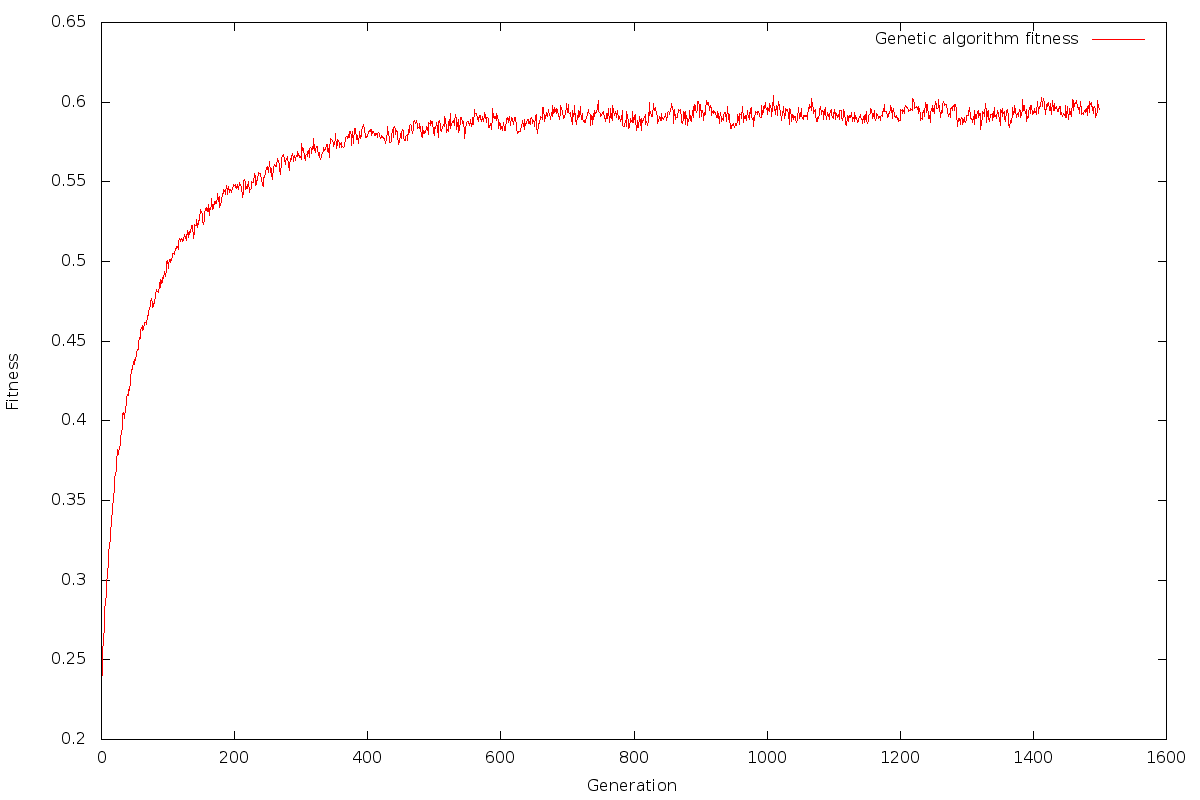
\includegraphics[width=\textwidth]{img/logcurve.png}
\caption{Curva logaritmica relativa al fitness dell'algoritmo genetico.}
\end{figure}
Dalle varie esecuzioni si può notare come la curva logaritmica dell'algoritmo
evolutivo sia limitata ad un punto\footnote{circa il 63\% per un'improvvisazione
di 12 misure con 1500 generazioni e 512 individui per generazione},
questo è un comportamento voluto
per essere in modo esplicito distanti dal concetto di riproduzione fedele di una
determinata composizione, rendendo quindi il tutto, in un certo modo,
simile alla composizione iniziale.
